%!TEX root = ../dissertation.tex

\chapter{Background}
\label{chap:background}
This chapter will provide brief background information about different types of physics studied in this manuscript. These include the dynamics of fluids, rigid and flexible multibody systems. Lastly, methods concerning the coupling between fluids and solids are discussed as well.

\section{Computational Fluid Dynamics}
Computational fluid dynamics is a significant branch of computational continuum mechanics, and it is concerned with the simulation of continua using computers. Many aspects of CFD have been studied in the past. This includes various space discretization and time integration schemes. Insofar as the space discretization step is concerned, the majority of CFD models can be classified as: $(i)$ Eulerian approaches, where the unknown state variables are attached to stationary observers; or $(ii)$ Lagrangian approaches, in which the unknown state variables are attached to moving observers.

Eulerian methods have been successfully applied and are very popular in CFD. Indeed, Finite Difference (FD) represents a robust technique for solving partial differential equations on simple domains, while the Finite Volume (FV) has been predominantly applied in fluid flows with complex geometries. Conversely, the Lagrangian methods gained traction only about two decades ago, although the idea of using Lagrangian discretization dates back to 1957 \cite{PIC}. Among Lagrangian methods, SPH  \cite{Lucy1977,Gingold1977} has been widely adopted as the low-order approximation of choice for a variety of problems \cite{Monaghan2005a}, while Moving Least Squares and Radial Basis Functions emerged as the leading high-order meshless methods \cite{trask2016compact,hu2019spatially,trask2018compatible,kansa1990scattered}. 

For FSI problems, just as for free-surface flows, the Eulerian approaches are challenged by large mesh deformations, which call upon re-meshing operations. A widely used approach is the Arbitrary Lagrangian-Eulerian (ALE) method \cite{ALE1974}, which handles well sufficiently small mesh deformation, yet it becomes expensive when the motion of the solid objects is relatively large. The Immersed Boundary Method (IBM) \cite{Peskin1977} addresses this shortcoming by implicitly treating the solid objects, as opposed to the ALE explicit representation of solid bodies that calls for body-fitted meshing. Thus, IBM alleviates the mesh deformation problem at the cost of a higher mesh resolution in the vicinity of the solid objects. 

Handling FSI problems comes more naturally to meshless methods, e.g. SPH, owing to their Lagrangian nature that interfaces well with the Lagrangian framework used in solid mechanics. However, SPH-based methods generally have enjoyed a somewhat limited adoption due to their reduced order and deficiencies in numerical approximation near boundaries \cite{trask2016compact}. Kernel-correction methods have been recently proposed to enforce linear consistency and second-order accuracy, yet they alter the conservation properties of SPH \cite{fatehi2011,Libersky1993,randles1996,Trask2015,islam2018consistency}. Likewise, the use of larger support basis functions improves robustness but leads to a higher computational cost.

Amongst different choices of discretization methods, in this thesis, SPH is embraced for space discretization of the underlying equations owing to its strength in solving free-surface, large-deformation, and fluid-solid interaction problems. SPH comes in many different formulations as far as time-integration, compressibility level, and boundary condition treatment are concerned, which will be further discussed in later chapters.



\section{Computational Multibody Dynamics}
A multibody system is defined as a collection of bodies interacting through mechanical constraints and frictional contact between the objects. Joints constrain the relative motion of bodies while springs and dampers induce additional loads in the system. Each body posses a specific mass and shape while the interconnects are treated as massless. These modeling assumptions apply to a large class of mechanical systems, from robots and vehicles to biomechanical systems \cite{simeon2013computational}. Computational multibody dynamics is the term used herein to refer to the numerical modeling technique used for resolving the dynamics of these discrete systems. Depending on the stiffness of discrete objects being studied, multibody systems may be further categorized into rigid multibody systems and flexible multibody systems.
\subsection{Rigid Multibody Systems}\label{sec:back_rigid}
A large body of literature is dedicated to rigid multibody systems featuring mechanical joints/constraints \cite{Haug89,shabana2013}. When frictional-contact between objects  is present, existing methods may be categorized in two groups: \textit{penalty} and \textit{complementarity} methods.

In penalty methods, the fundamental assumption is that bodies, although being rigid, deform slightly at the point of contact. The inter-penetration between the rigid bodies calculated during the proximity-computation stage is used to penalize further inter-penetration by creating contact forces between bodies through fictitious springs and dampers \cite{cundall71,cundall79,cundall1988formulation}. The process of choosing the model parameters and the simplification of the contact geometry are two main drawbacks of this method. Despite its shortcomings, penalty method has been used in numerous numerical studies on the dynamics of large rigid body systems \cite{Jaeger1996,brilliantov1996model,vu1999elastoplastic,vu2004accurate,luding2005,poschel2005computational}.

In the complementarity (constraint-based) approach, the main idea is to modify the equations of motion to include a differential inclusion \cite{filippov1967classical} and to impose non-penetration between rigid bodies through constraints enforced by applying impulses.  This method has been modified to model rolling and spinning friction in addition to sliding friction \cite{AleMihaiFriction2013}.  An important drawback associated with this method is the lack of uniqueness in the set of contact forces resulting from the solution of an optimization problem. In the present work, the complementarity method is employed to resolve the dynamics of contact between rigid bodies, while the penalty approach is used to handle contact between deformable bodies.


\subsection{Flexible Multibody Systems}
Unlike the rigid body dynamics where there is no distinction between the kinematics of the body and its reference frame, further modeling is required to capture the deformation of elastic components in flexible body dynamics. This is mainly because the distance between two points on/inside a deformable body changes, and the kinematics of the reference frame cannot sufficiently describe the time evolution of the flexible component. To this end, elastic components are discretized in space to study their motion via a \textit{finite} number of degrees of freedom. This is in contrast to rigid multibody systems where each rigid object is uniquely defined, regardless of its shape, by a set of position and orientation degrees of freedom. The final stage of the solution consists of solving for state variables, including those associated with rigid body motion as well as those defining elastic displacements and/or position and orientation of the discretized nodes.  The Floating Frame of Reference (FFR), co-rotational formulation, and Absolute Nodal Coordinate Formulation (ANCF) are three of the most relevant formulations in the context of flexible multibody systems. 


In the FFR formulation, the position of a point in the flexible body is expressed as the superposition of a small (flexible) \textit{deformation}, described in the body coordinate system, and possibly large \textit{translation} and \textit{rotation} of the body's coordinate system. The deformation of the body with respect to its coordinate system is expressed via the nodal coordinates of the discretized finite elements. The finite element used in the FFR formulation leads to zero strain under any arbitrary rigid body motion of the flexible object. Despite being the most widely used formulation in the computational flexible body dynamics, FFR is limited to cases where the deformation of the flexible body with respect to its reference frame is small. See \cite{Shabana1997,TR-2016-05-Recuero} for more details about the FFR formulation.  

The ANCF is a non-linear finite element method formulated to handle large deformations. In ANCF, no co-rotated frame is used to describe the kinematics of deformed finite elements. Most importantly, the distinguishing feature of ANCF is the use of position vector gradients to describe the rotation of the body as well as its strain state, thereby avoiding the need for interpolating non-vectorial rotation parameters. Given the interest of the present work in problems featuring large deformations and driven by the limitations of the FFR for such problems, the ANCF method is chosen in the present work. 


\section{Fluid-Solid Interaction}\label{sec:FSI_intro}
Many engineering applications, e.g., cardiovascular flows, fluid sloshing, particles in suspension, etc., require the solution of an FSI problem. Some of these problems involve large deformations, in which case the fluid-solid coupling remains challenging to solve \cite{ryzhakov2010}. For most FSI problems, it is nearly impossible to obtain analytical solutions. Additionally, laboratory experiments are also limited and costly to conduct \cite{hou2012}. Thus, numerical simulations must be employed. Different classifications exist in the context of numerical methods for FSI problems.

One classification is to consider the computational domain and divide the methods into \textit{conforming mesh methods} and \textit{non-conforming mesh methods}. In the conforming mesh methodology, the computational domains of sub-systems match at the interface, while in non-conforming mesh methods the computational domain of the fluid sub-system serves more as a background mesh for the solid phase. As an example of non-conforming mesh methods, in IBM \cite{peskin2002,mittal2005immersed}, the immersed boundary is tracked in a Lagrangian fashion; the fluid is tracked in an Eulerian framework on a non-conforming and regular grid; lastly, the presence of the immersed boundary on the non-conforming grid is included in Navier-Stokes equations as extra source terms. Fig.~\ref{fig:FSI_lit} illustrates the difference between the computational domains of the aforementioned methods. The approach to be taken in the current work does not fit into this classification since a mesh-less method is to be used for the fluid phase. However, the methodology is more similar to conforming mesh methods.

\begin{figure}[t!]
	\centering
	\begin{subfigure}[t]{0.4\textwidth}
		\centering
		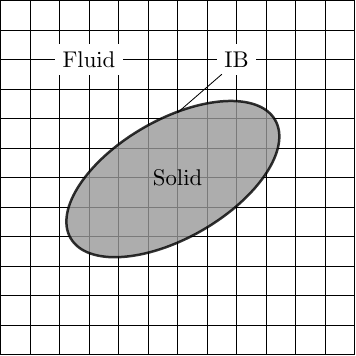
\includegraphics[width=1\linewidth]{images/IBM.png}
		\caption{Non-conforming mesh method in IBM}
	\end{subfigure}%
	~ 
	\begin{subfigure}[t]{0.5\textwidth}
		\centering
		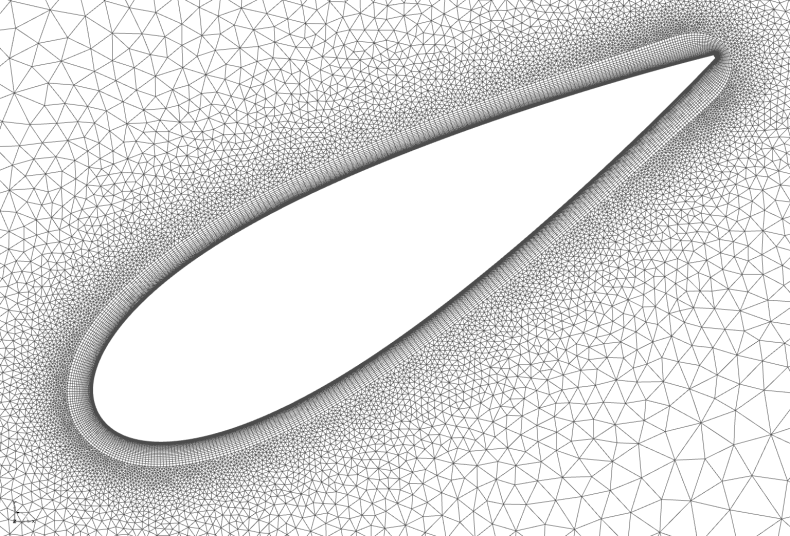
\includegraphics[width=1\linewidth,height=0.8\linewidth]{images/ConformingMesh.png}
		\caption{Conforming mesh method}
	\end{subfigure}
\caption{Illustration of the computational domains for non-conforming and conforming mesh methods.}
\label{fig:FSI_lit}
\end{figure}

Another classification pertains to the sequence of the solution algorithms and the governing equation of the overall system. Accordingly, FSI methods are grouped  into \textit{monolithic} and \textit{partitioned} approaches. In the former \cite{hubner2004,ryzhakov2010,michler2004}, the governing equations of the fluid and the solid phases are solved simultaneously; the interfacial conditions are implicit in the solution procedure; and potentially a better accuracy can be obtained for a multidisciplinary problem \cite{hou2012}. In contrast, in the latter approach, the two phases are solved separately, and the solutions are usually explicitly coupled together. Each method has its advantages and drawbacks. What makes the partitioned approach appealing is the fact that it solves each phase with efficient techniques that make the most out of the state-of-the-art methods in modeling, numerical solvers, and hardware architectures. Among partitioned methods, the ALE approach for the fluid and Lagrangian one for the solid are commonly used to treat strongly-coupled FSI problems \cite{hughes1981,souli2000}. In the ALE approach, the fluid mesh is deformed to adapt to the solid domain deformation \cite{fourey2010}. Although this approach has proven capable of handling  FSI problems with large-deformations, it is computationally expensive due to continuous mesh adaptation, a task that is not needed in meshless Lagrangian methods such as SPH \cite{yang2012}. 


Some recent FSI schemes resolve both the solid and the fluid dynamics in an Eulerian framework \cite{valkov2015eulerian,kamrin2012reference, liu2001eulerian,miller2002conservative}. The difficulty of computing the deformation gradient in an Eulerian framework is circumvented by tracking a reference map \cite{valkov2015eulerian,kamrin2012reference} or direct evolution of the deformation gradient as a field variable \cite{liu2001eulerian}. A distinct advantage of this class of methods is that all the phases are resolved by sweeping through a single mesh. On the downside, these methods are challenged by FSI problems involving contact between a large number of solid bodies as the computation of contact forces requires two level-set field variables per contact. Storing these field variables becomes expensive in comparison to $O(1)$ state variables that are stored in Lagrangian formulations \cite{valkov2015eulerian} for each contact.

In the present research, the Fluid-Solid Interaction method will be resolved in a Lagrangian-Lagrangian framework. Similar fluid-structure coupling was discussed in \cite{attaway1994} and further improved in \cite{fourey2010,Vuyst2005,groenenboom2010}. In \cite{attaway1994}, the contact forces were calculated based on an iterative master-slave scheme, which finds the best penalty forces required for the no-penetration condition. A similar but non-iterative scheme was used in \cite{groenenboom2010}. In \cite{fourey2010,armanCompFluids2015}, a dummy-particles scheme was used to compute the pressure from the fluid side. The present work follows in the footsteps of this last approach. 







\section{Granular Flows}\label{sec:back_granular}
While water is the most handled industrial material, granular material is the second.  Dense granular flows, however, are substantially more complex than their fluid counterparts. Granular material is essentially a discrete system whose evolution is described by the Newton-Euler's equations featuring frictional contact force (see Eq.~\ref{eq:Newton_Euler}). Although the discrete representation can accurately capture the motion of granular flows, the fully resolved modeling of large scale granular flows is a challenging task owing to $(i)$ their complex frictional contact interactions, and $(ii)$ a high computational burden as the motion of individual particles needs to be tracked in a numerical integration framework that advances simulation at time steps $\Delta t \approx 10^{-5}$ or lower. To address the latter aspect, discrete granular flow simulations use parallel computing to accelerate the computations. To date, the largest granular dynamics simulation of practical relevance contained 2.4 billion bodies, which was run on 16,384 CPUs (131,072 cores) of Japan's K-computer \cite{billBodyDEMJapanSC2017,japanDEMlarge2018}, the 2012 fastest supercomputer in the world and now the 18th in the ranking of the world's supercomputers \cite{TOP500}.

The collective behavior of individual particles may, however, be regarded as a continuum. Given that granular media can demonstrate distinctively different behaviors under various local stress conditions, the focus of this research is on the fluid-like evolution of granular material that happens when it is rapidly sheared. In such cases, $(i)$ shear stress in granular material shows strain-rate dependency, which is a characteristic of fluids and, $(ii)$ there exists a threshold value (yield criterion), under which the grains do not flow, a characteristic of solid materials. These features suggest a viscoplastic behavior of a granular material which is similar in nature to that of non-Newtonian fluids such as Bingham liquids \cite{jop2006constitutiveNature,campbell1990rapid}. 

Constitutive laws that could describe the motion of granular flows are still lacking. Amongst various models and theories developed previously, the $\mu(I)$-rheology \cite{jop2006constitutiveNature} is one of the successful frameworks describing observations from a variety of experimental and numerical results.

In the present work, we describe the fully resolved modeling of granular flows via the complementarity approach described in \S\ref{sec:back_rigid}.